\section{Results}
\begin{frame}
  \frametitle{Flow of Pure Solvent}
%   \begin{itemize}
%   \item Initial condition: ``seed'' vapor particles in the center of
%     the domain
%   \item Domain is periodic, edges of the domain $T=T_s +
%     \Delta T$
%   \item Theory predicts a self similar temperature profile $T =
%     T(r/R(t))$, where $r$~---~distance from the center, $R(t)$~---~radius of
%     the bubble
%   \end{itemize}

\begin{figure}
    \centering
    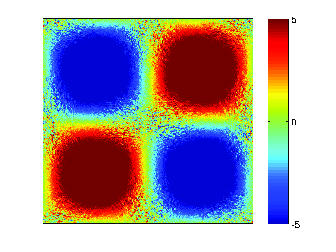
\includegraphics[width=0.5\textwidth]{img/polymer_loc-15.png}
    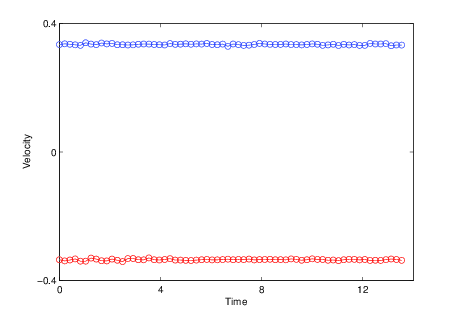
\includegraphics[width=0.5\textwidth]{img/polymer_loc-9.png}
    \caption{Vorticity field and velocity of one point in flow of pure solvent flow at $Re\approx 80$.}
    \label{fig:vor_sol}
  \end{figure}
\end{frame}

\begin{frame}
  \frametitle{Flow of Polymer Solution}
  \begin{figure}
    \centering
    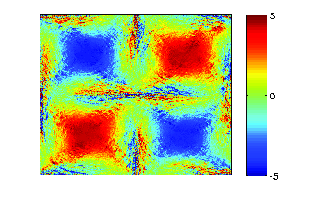
\includegraphics[width=0.6\textwidth]{img/polymer_loc-10.png}
  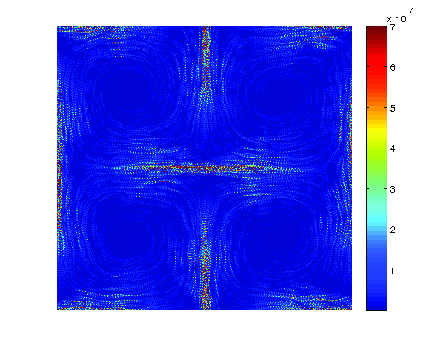
\includegraphics[width=0.5\textwidth]{img/polymer_loc-6.png}
    \caption{Vorticity field and elastic stress trace in flow of polymer solution at $Wi\approx1$.}
    \label{fig:vor_pol1}
  \end{figure}
\end{frame}

\begin{frame}
  \frametitle{Flow of Polymer Solution}
\begin{figure}[ht]
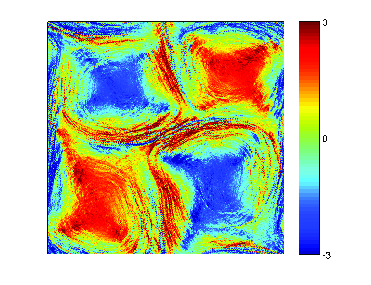
\includegraphics[width=0.5\textwidth]{img/polymer_loc-12.png}
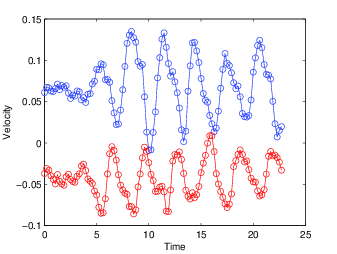
\includegraphics[width=0.5\textwidth]{img/polymer_loc-7.png}
\caption{Vorticity field and velocity of one point in flow of polymer solution at $Wi\approx5$.}
\label{fug:vor_pol5}
\end{figure}
\end{frame}
% \begin{frame}
%   \frametitle{Flow of Polymer Solution}
%   \begin{figure}[ht]
% 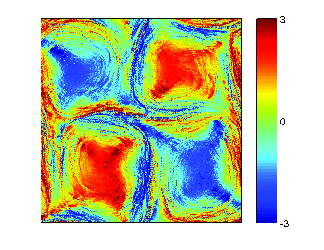
\includegraphics[width=0.5\textwidth]{img/polymer_loc-13.png}
% 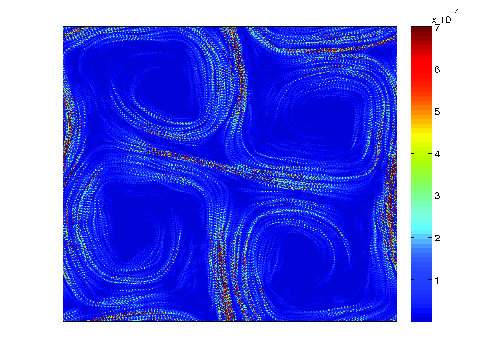
\includegraphics[width=0.5\textwidth]{img/polymer_loc-5.png}
% \caption{Velocity and elastic stress trace in flow of polymer solution at $Wi\approx5$.}
% \label{fug:vel_pol5}
% \end{figure}
% \end{frame}
\begin{frame}
  \frametitle{Flow of Polymer Solution}
  \begin{figure}[ht]
    \centering
    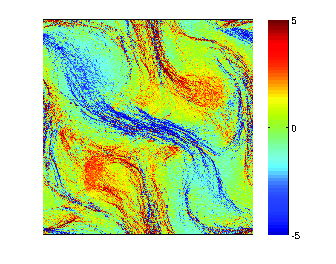
\includegraphics[width=0.5\textwidth]{img/polymer_loc-14.png}
    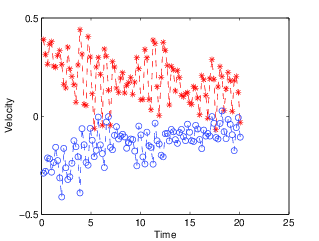
\includegraphics[width=0.5\textwidth]{img/polymer_loc-8.png}
    \caption{Vorticity field and velocity of one point in flow of polymer solution at $Wi\approx10$.}
    \label{fig:vor_pol10}
  \end{figure}
\end{frame}

\begin{frame}
 \frametitle{Flow of Polymer Solution}
  \begin{figure}[t]
    \centering
    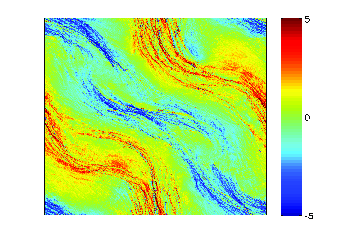
\includegraphics[width=0.5\textwidth]{img/polymer_loc-11.png}
 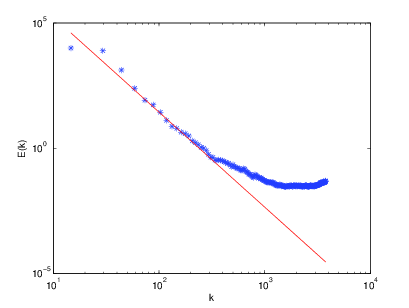
\includegraphics[width=0.5\textwidth]{img/polymer_loc-0.png}
    \caption{Vorticity field and energy spectrum in flow of polymer solution at $Wi\approx10$ with perturbation.}
    \label{fig:vor_per}
  \end{figure}
\bibliographystyle{elsart-num}
\nobibliography{bibdata}
\end{frame}

%%% Local Variables: 
%%% mode: latex
%%% TeX-master: t
%%% End: 
